\chapter{Descripción}\label{chapter03}

AIVA es un sistema web orientado a pequeñas y medianas empresas de alimentos perecederos, como por ejemplo panaderías y confiterías, que busca reducir mermas y quiebres de stock mediante la planificación de producción y reposición basada en datos. La propuesta integra, en una única plataforma, la captura flexible de ventas (punto de venta, importación de CSV y carga asistida por imágenes), el enriquecimiento contextual (clima, calendario y patrones semanales) y un módulo de predicción de demanda diaria por producto. Sobre esta base, el sistema ofrece visualizaciones ejecutivas (backoffice), un asistente conversacional para consultas operativas y un mecanismo de alertas que anticipa situaciones de sobreproducción o faltantes. 

El núcleo analítico del sistema combina el historial transaccional con variables exógenas para estimar la demanda esperada a corto plazo. Este módulo implementa un enfoque heurístico transparente centrado en tendencia, estacionalidad y condiciones meteorológicas, con un diseño abierto a la incorporación de modelos estadísticos y de aprendizaje automático más avanzados. La arquitectura prioriza componentes de bajo costo y rápida adopción, asegurando trazabilidad de datos, reproducibilidad de resultados y una experiencia de usuario alineada con los flujos cotidianos del negocio.

\vspace{1cm}


\section{Funcionalidades del sistema}

\begin{itemize}
    \item \textbf{Autenticación y perfiles de usuario}
    \begin{itemize}
        \item Registro e inicio de sesión mediante servicio gestionado (Supabase Auth).
        \item Persistencia de sesión y provisión de identidad a la aplicación.
        \item Gestión básica de perfil de usuario.
    \end{itemize}

    \item \textbf{Configuración y localización}
    \begin{itemize}
        \item Inicialización de la ubicación del usuario (por defecto, Ciudad Autónoma de Buenos Aires).
        \item Persistencia de la ubicación para consumo por servicios externos (clima).
    \end{itemize}

    \item \textbf{Gestión de productos y categorías}
    \begin{itemize}
        \item Crear, leer, actualizar y eliminar productos y categorías.
        \item Carga masiva de productos vía CSV con previsualización y validación básica.
        \item Ajustes manuales de stock y visualización de movimientos de stock.
    \end{itemize}

    \item \textbf{Registro y administración de ventas}
    \begin{itemize}
        \item Punto de Venta (POS): Flujo de carrito, totales y confirmación de venta. Alta de venta y detalle de ítems en base de datos. Enriquecimiento contextual de cada transacción para análisis de demanda.
        \item Importación de ventas históricas (CSV): Carga de archivos CSV con validaciones y normalización.
        \item Carga asistida por imágenes (OCR): Interfaz de carga y estados de procesamiento.
    \end{itemize}

    \item \textbf{Datos contextuales de clima}
    \begin{itemize}
        \item Integración con API meteorológica.
        \item Disponibilización de variables climáticas para análisis y predicción.
    \end{itemize}

    \item \textbf{Análisis de demanda}
    \begin{itemize}
        \item Consolidación de datos transaccionales enriquecidos.
        \item Consultas y visualizaciones exploratorias (tendencias por producto/categoría, comparativas temporales).
    \end{itemize}

    \item \textbf{Predicción de demanda}
    \begin{itemize}
        \item Generación de predicciones: Estimación diaria por producto mediante enfoque heurístico (tendencia, estacionalidad, día de semana y clima). Indicadores asociados a cada predicción.
        \item Persistencia y consulta de predicciones: Almacenamiento de predicciones para trazabilidad y auditoría. Gráficos comparativos entre predicción y ventas observadas.
        \item Predicciones resumidas para tableros: Consolidación de resultados para consumo eficiente por el dashboard.
    \end{itemize}

    \item \textbf{Backoffice (dashboard)}
    \begin{itemize}
        \item Indicadores ejecutivos (ventas, productos destacados, clima, predicciones vigentes).
        \item Visualizaciones de gráficos con filtros para seguimiento operativo.
    \end{itemize}

    \item \textbf{Reportes}
    \begin{itemize}
        \item Generación de reportes con agregados por período, producto y categoría.
        \item Gráficos de evolución y comparativas semana a semana.
    \end{itemize}

    \item \textbf{Alertas operativas}
    \begin{itemize}
        \item Listado de alertas de referencia (p. ej., stock bajo, sobreproducción potencial, feriados).
        \item Priorización de casos para acción correctiva.
    \end{itemize}

    \item \textbf{Asistente conversacional}
    \begin{itemize}
        \item Interfaz de chat para consultas frecuentes y navegación guiada.
        \item Respuestas basadas en reglas; integración con modelos de lenguaje planificada.
    \end{itemize}

    \item \textbf{Gestión de planes y suscripciones}
    \begin{itemize}
        \item Plan gratuito por defecto y soporte para planes pagos.
        \item Asociación de usuarios a planes y consulta del estado de suscripción.
    \end{itemize}

    \item \textbf{Perfil y preferencias}
    \begin{itemize}
        \item Edición de datos básicos de perfil.
        \item Configuraciones generales del usuario.
    \end{itemize}

    \item \textbf{Validaciones y manejo de errores}
    \begin{itemize}
        \item Validación de formularios y archivos (CSV).
        \item Mensajería de estados (carga, éxito, error) y prevención de acciones inválidas.
    \end{itemize}

    \item \textbf{Seguridad y segmentación de datos}
    \begin{itemize}
        \item Acceso autenticado a recursos y filtrado de datos por usuario.
        \item Preparado para políticas de control a nivel base de datos (RLS) en despliegues gestionados.
    \end{itemize}
\end{itemize}

\vspace{1cm}
\section{Tecnologías utilizadas}\label{sec:tecnologias}
A continuación se detallan las tecnologías empleadas en AIVA, explicando su rol dentro de la solución, el modo de integración y los criterios que justifican su elección. La selección prioriza un balance entre rapidez de implementación, bajo costo operativo, mantenibilidad y adecuación a los requerimientos del sistema.

\subsection{Next.js (React + TypeScript)}
Next.js es un \textit{framework} sobre React que incorpora enrutamiento, optimizaciones de rendimiento y opciones de renderizado (cliente/servidor). En AIVA se utiliza para:
\begin{itemize}
    \item Implementar la interfaz web con componentes reutilizables y tipado estático (TypeScript), reduciendo defectos en tiempo de compilación.
    \item Organizar el ruteo (App Router) separando vistas operativas (\textit{dashboard}, POS, predicción, reportes) de páginas auxiliares (autenticación, perfil).
    \item Favorecer una arquitectura mantenible (módulos, \textit{hooks} y servicios) con buena escalabilidad del frontend.
\end{itemize}
\noindent\textbf{Motivación.} Ecosistema maduro y documentación extensa, compatible con librerías modernas de UI.

\subsection{Tailwind CSS y \textit{shadcn/ui}}
Tailwind CSS provee utilidades de estilo de bajo nivel; \textit{shadcn/ui} aporta componentes accesibles basados en Tailwind.
\begin{itemize}
    \item Permiten maquetar formularios, tablas, modales y gráficos con consistencia visual y tiempos de desarrollo acotados.
    \item Estandarizan patrones de interacción (validaciones, estados de carga y error) y facilitan la personalización fina del diseño.
\end{itemize}
\noindent\textbf{Motivación.} Coherencia visual y productividad. 

\subsection{Recharts}
Recharts es una biblioteca de gráficos para React.
\begin{itemize}
    \item Se utiliza en el \textit{dashboard} y reportes para visualizar KPIs (ventas por período, productos destacados) y comparativas (predicción vs.\ observado).
    \item Ofrece componentes responsivos y composables, adecuados para vistas con filtros interactivos.
\end{itemize}
\noindent\textbf{Motivación.} Integración directa con React y bajo costo de aprendizaje.

\subsection{Supabase Auth}
Servicio gestionado para registro, inicio de sesión y manejo de sesiones (incluida verificación por correo).
\begin{itemize}
    \item Centraliza la identidad del usuario y emite \textit{tokens} para acceder a recursos protegidos.
    \item Simplifica la implementación de rutas seguras y del \textit{feature gating} por plan/suscripción.
\end{itemize}
\noindent\textbf{Motivación.} Reduce superficie de error y esfuerzo de mantenimiento respecto de una solución propia.

\subsection{PostgreSQL (vía Supabase)}
Base de datos relacional donde reside el modelo de datos.
\begin{itemize}
    \item Tablas operativas: \textit{products}, \textit{categories}, \textit{sales}/\textit{sale\_items}, \textit{stock\_movements}.
    \item Datos analíticos y de contexto: \textit{demand\_analysis\_data}, \textit{predictions}/\textit{stored\_predictions}, \textit{weather\_data}, \textit{plans}, \textit{user\_subscriptions}.
    \item Soporte de integridad referencial, vistas e \textit{indexes} para consultas eficientes.
\end{itemize}
\noindent\textbf{Motivación.} Robustez y expresividad SQL para analítica operativa.

\subsection{PostgREST (Supabase)}
Capa que expone el esquema de PostgreSQL como API REST tipada.
\begin{itemize}
    \item La capa de servicios del frontend consume esta API para operaciones CRUD y consultas filtradas.
    \item Mantiene trazabilidad entre el modelo lógico y los endpoints, reduciendo código \textit{boilerplate}.
\end{itemize}
\noindent\textbf{Motivación.} Acelera la construcción de la capa de datos manteniendo convenciones REST.

\subsection{OpenWeatherMap API}
Fuente externa de variables meteorológicas usadas como factores exógenos.
\begin{itemize}
    \item Proporciona temperatura, estado del tiempo y otros atributos que se asocian a ventas y se persisten para análisis.
    \item Se contemplan \textit{fallbacks} ante indisponibilidad o latencia elevada.
\end{itemize}
\noindent\textbf{Motivación.} Cobertura suficiente para el ámbito del proyecto.

\subsection{Node.js y \texttt{npm}}
Entorno de ejecución y gestor de dependencias del proyecto.
\begin{itemize}
    \item Se emplea para el servidor de desarrollo, construcción del frontend y automatización de tareas (scripts).
    \item Estandariza \textit{linting}, empaquetado y gestión de versiones.
\end{itemize}
\noindent\textbf{Motivación.} \textit{Tooling} ampliamente adoptado en el ecosistema web.

\subsection{Utilitarios de CSV}
Conjunto de utilidades para ingesta histórica.
\begin{itemize}
    \item Validan formato, normalizan columnas y registran errores durante la carga de productos y ventas.
    \item Priorizan trazabilidad (filas aceptadas, rechazadas o corregidas) para reproducibilidad.
\end{itemize}
\noindent\textbf{Motivación.} Simplicidad y compatibilidad con exportaciones comunes.

\subsection{Buenas prácticas de configuración y seguridad}
\begin{itemize}
    \item Gestión de credenciales mediante variables de entorno (\texttt{.env}), evitando su versionado.
    \item Separación de entornos (desarrollo/producción) y rotación periódica de claves.
    \item En despliegues gestionados, aplicación de RLS por \textit{user\_id} para segmentación de datos.
\end{itemize}


\vspace{1cm}

\section{Diagrama de flujos}

Para describir el comportamiento dinámico del sistema incorporamos diagramas de flujo que muestran, paso a paso, cómo se procesan las operaciones clave. Estos esquemas complementan a los requerimientos y a la arquitectura estática, al hacer explícitas las secuencias, los puntos de decisión, los caminos alternativos y el manejo de errores, lo que facilita la validación funcional y el diseño de casos de prueba.
\vspace{1cm}


\subsection{DF-A · Autenticación}
El diagrama modela el control de acceso y el alta de usuarios. Se definió así para equilibrar seguridad (validaciones en el servicio de autenticación y verificación de correo), usabilidad (separación clara entre registro e inicio de sesión) y recuperabilidad (manejo de errores con retroalimentación inmediata). La convergencia final en el dashboard establece un único criterio de éxito y facilita la trazabilidad de estados; el objetivo es registrar las decisiones críticas del acceso sin describir pantallas intermedias.

\begin{figure}[!htbp]
  \centering
  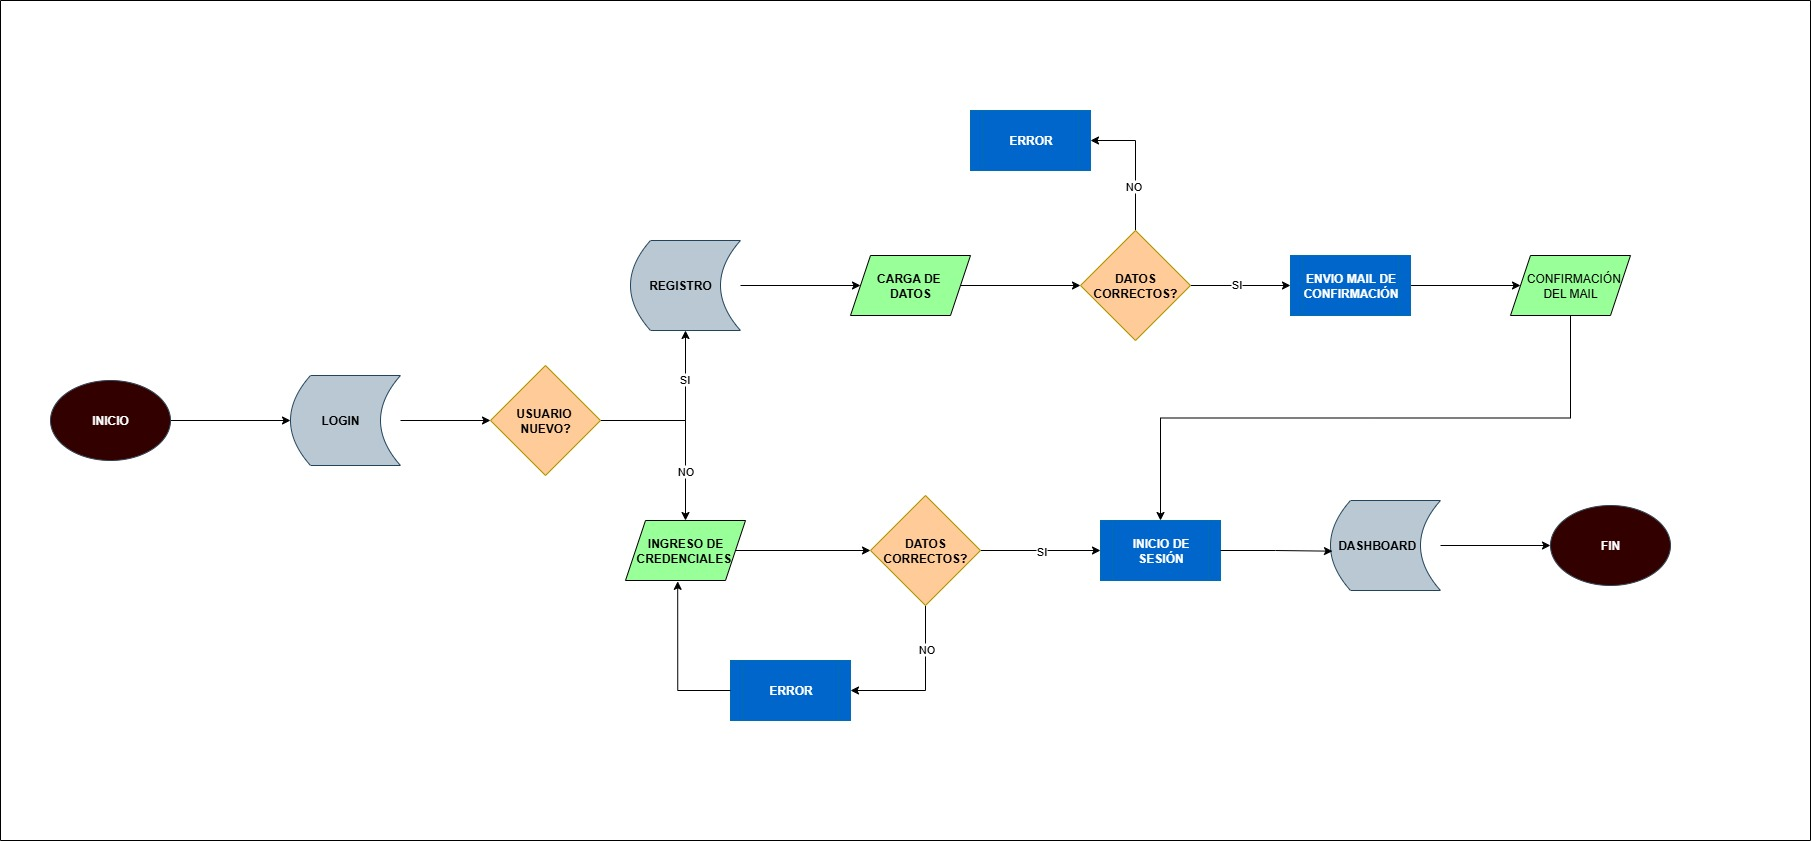
\includegraphics[width=0.92\textwidth]{images/FlujoAutenticacion.jpg}
  \caption{DF-A · Autenticación -- Fuente: elaboración propia}
  \label{fig:df-a-autenticacion}
\end{figure}


\subsection{DF-B · Carga de ventas}
El diagrama describe el proceso de registro de ventas desde dos orígenes complementarios: ingreso manual tipo POS y carga automática (OCR/CSV). Se define así para cubrir los escenarios operativos más frecuentes con validaciones progresivas y una confirmación explícita antes del alta, incorporando puntos de corrección para minimizar errores y preservar trazabilidad. La bifurcación temprana optimiza tiempos según la fuente de datos y el cierre en confirmación establece una única condición de éxito.

\begin{figure}[!htbp]
  \centering
  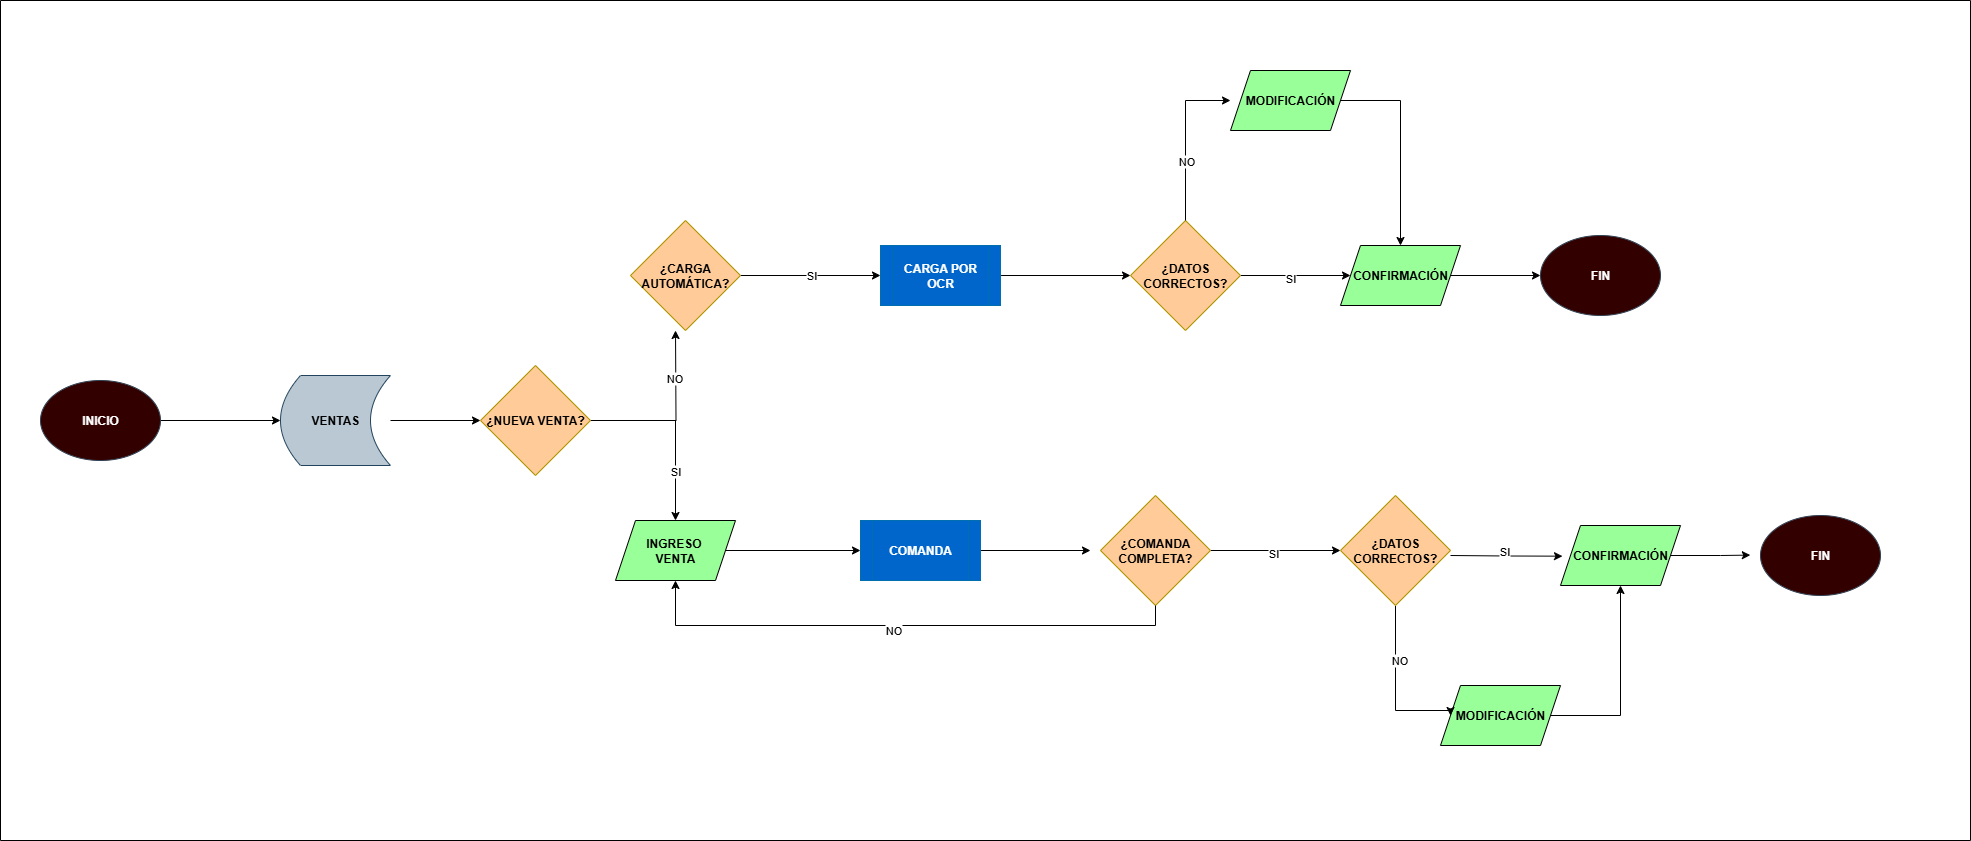
\includegraphics[width=0.92\textwidth]{images/FlujoVentas.drawio.png}
  \caption{DF-B · Carga de ventas -- Fuente: elaboración propia}
  \label{fig:df-b-ventas}
\end{figure}


\subsection{DF-C · Planes y suscripciones}
El diagrama describe la gestión de planes dentro de la aplicación. Al crear una cuenta, el usuario recibe automáticamente el plan gratuito; por este motivo, cualquier cambio de plan se realiza exclusivamente desde la app. El flujo contempla verificación de identidad y estado de suscripción, selección del nuevo plan y confirmación (incluida la validación de pago si corresponde). Ante éxito se actualiza la suscripción y se reflejan las capacidades en sesión; ante error se conserva el plan previo. El enfoque prioriza control de acceso, trazabilidad y una transición segura entre planes.

\begin{figure}[!htbp]
  \centering
  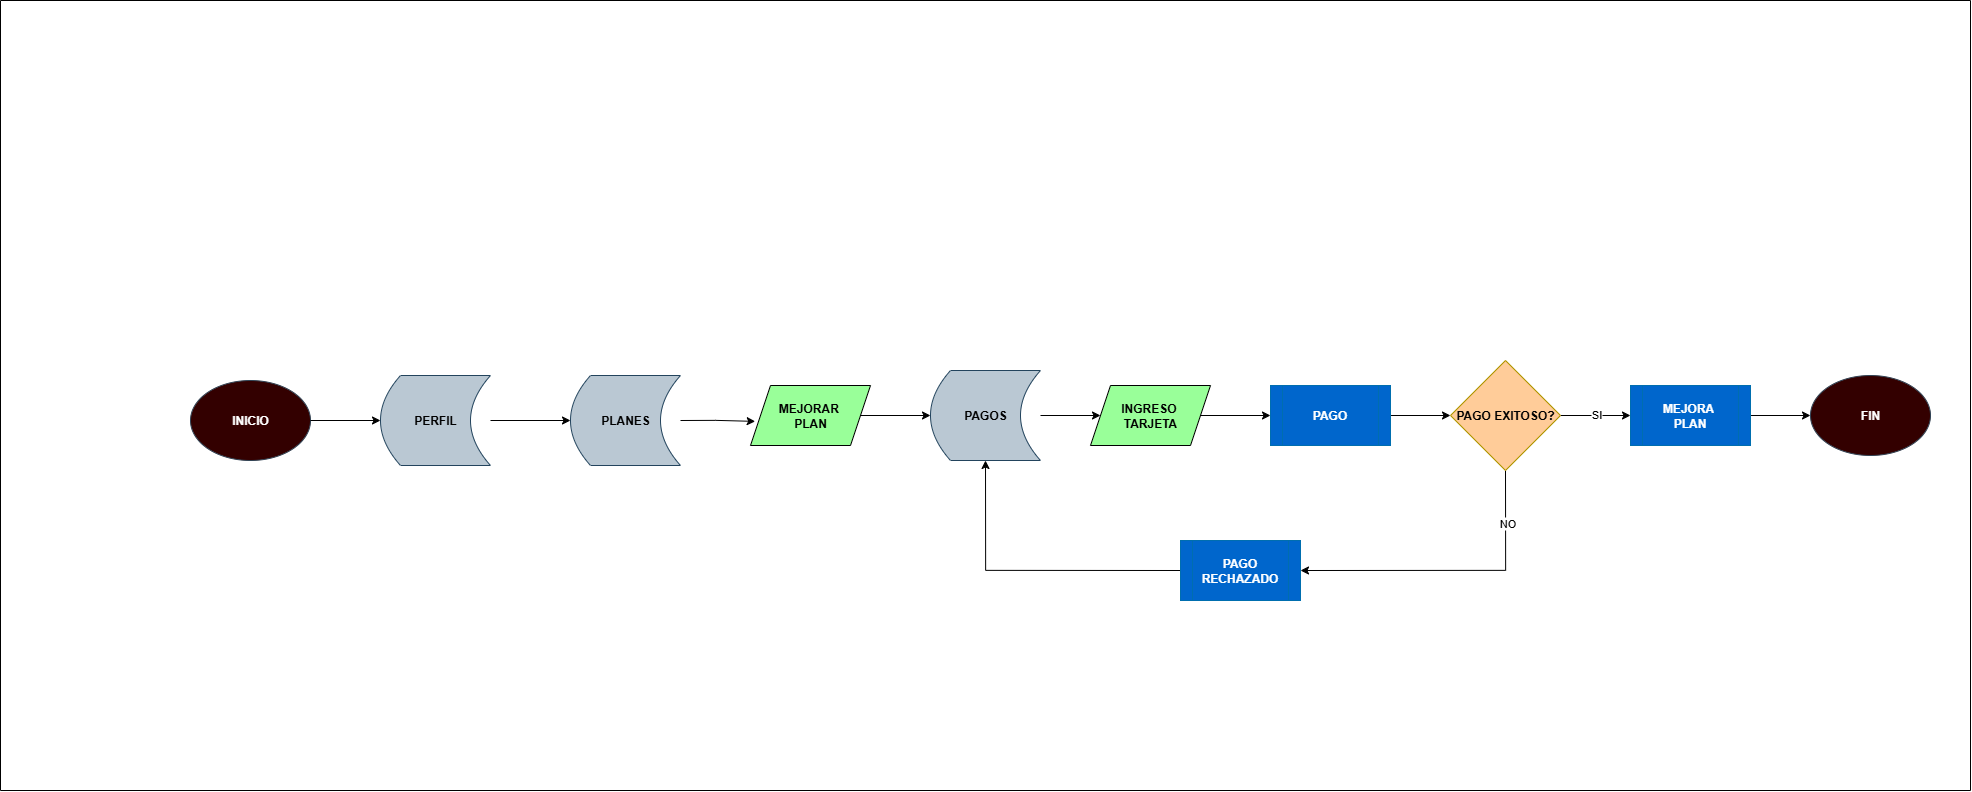
\includegraphics[width=0.92\textwidth]{images/FlujoPlanes.drawio.png}
  \caption{DF-C · Planes y suscripciones -- Fuente: elaboración propia}
  \label{fig:df-c-planes}
\end{figure}


\vspace{1cm}
\section{Identidad de marca}\label{sec:brand}

La identidad de marca de \textbf{AIVA} se diseñó para comunicar tecnología confiable, simplicidad operativa y foco en pequeños comercios. Esta sección documenta los elementos rectores de esa identidad y su relación con la experiencia de uso del sistema.

\subsection{Naming}
\textbf{AIVA} es un acrónimo de \textit{Asistente Inteligente para Ventas y Análisis}. El nombre cumple tres criterios: (i) \textit{memorabilidad} y pronunciación sencilla en español e inglés, (ii) \textit{brevedad} apta para interfaces y piezas breves (íconos, botones, navegación), y (iii) \textit{connotación} directa con analítica y apoyo a la decisión. El nombre se usa en mayúsculas para reforzar la legibilidad y la consistencia visual en la interfaz.

\subsection{Misión}
Poner la analítica predictiva al alcance de micro y pequeñas empresas de alimentos perecederos, reduciendo mermas y quiebres mediante planificación basada en datos. La misión orienta decisiones de producto hacia soluciones de bajo costo, fáciles de adoptar y con impacto operativo medible.

\subsection{Visión}
Constituirse en la plataforma de referencia en América Latina para la gestión de demanda en comercios de proximidad, integrando múltiples fuentes de datos (histórico, clima, calendario) y promoviendo prácticas sustentables de producción y reposición.

\subsection{Paleta de colores}\label{subsec:paleta}

La paleta cromática de \textbf{AIVA} fue definida para comunicar confianza tecnológica, claridad y foco en la toma de decisiones. El eje visual está compuesto por un rango de azules–índigo que se aplica en fondos y navegación, desde un índigo profundo hasta un azul más luminoso (\#1E2A78–\#3F6BFF). Esta base fría evoca precisión y estabilidad, atributos propios de una plataforma analítica, y refuerza la percepción de fiabilidad por parte del usuario.

Como acento de marca se incorpora el violeta (\#7C3AED, con su variante clara \#A78BFA), que introduce una connotación de innovación y modernidad. Este matiz se reserva para elementos de énfasis —botones primarios, indicadores destacados y piezas de comunicación—, logrando contraste visual sin perder coherencia con el tono profesional del sistema. Complementariamente, el cian (\#38BDF8) funciona como color informativo en enlaces y ayudas contextuales, guiando la atención sin distraer del contenido principal.

Los colores semánticos se emplean para codificar estados del sistema y facilitar la lectura operativa: el verde (\#22C55E) comunica confirmaciones y resultados positivos, mientras que el naranja (\#F59E0B) señala advertencias y situaciones que requieren seguimiento. La selección de saturación y brillo busca que estos mensajes sean perceptibles de forma inmediata, manteniendo, al mismo tiempo, una estética sobria adecuada al ámbito empresarial.

La familia de neutros se utiliza para garantizar legibilidad tipográfica y jerarquía en las superficies: un gris muy oscuro para textos (\#0F172A) y un gris claro para fondos (\#F1F5F9), complementados por blanco (\#FFFFFF) en componentes de alta claridad. En consonancia con pautas de accesibilidad, se privilegian combinaciones de alto contraste en las vistas más frecuentes, asegurando que la interfaz conserve nitidez tanto en entornos luminosos como en configuraciones de bajo brillo.

En conjunto, el gradiente principal de índigo a azul, el acento violeta y los semánticos verde/naranja construyen un lenguaje visual consistente: profesional en su base, expresivo en sus acentos y funcional en la comunicación de estados. Esta identidad cromática sostiene la experiencia de uso de AIVA y refuerza su posicionamiento como asistente inteligente para la gestión de demanda.

\begin{figure}[!htbp]
  \centering
  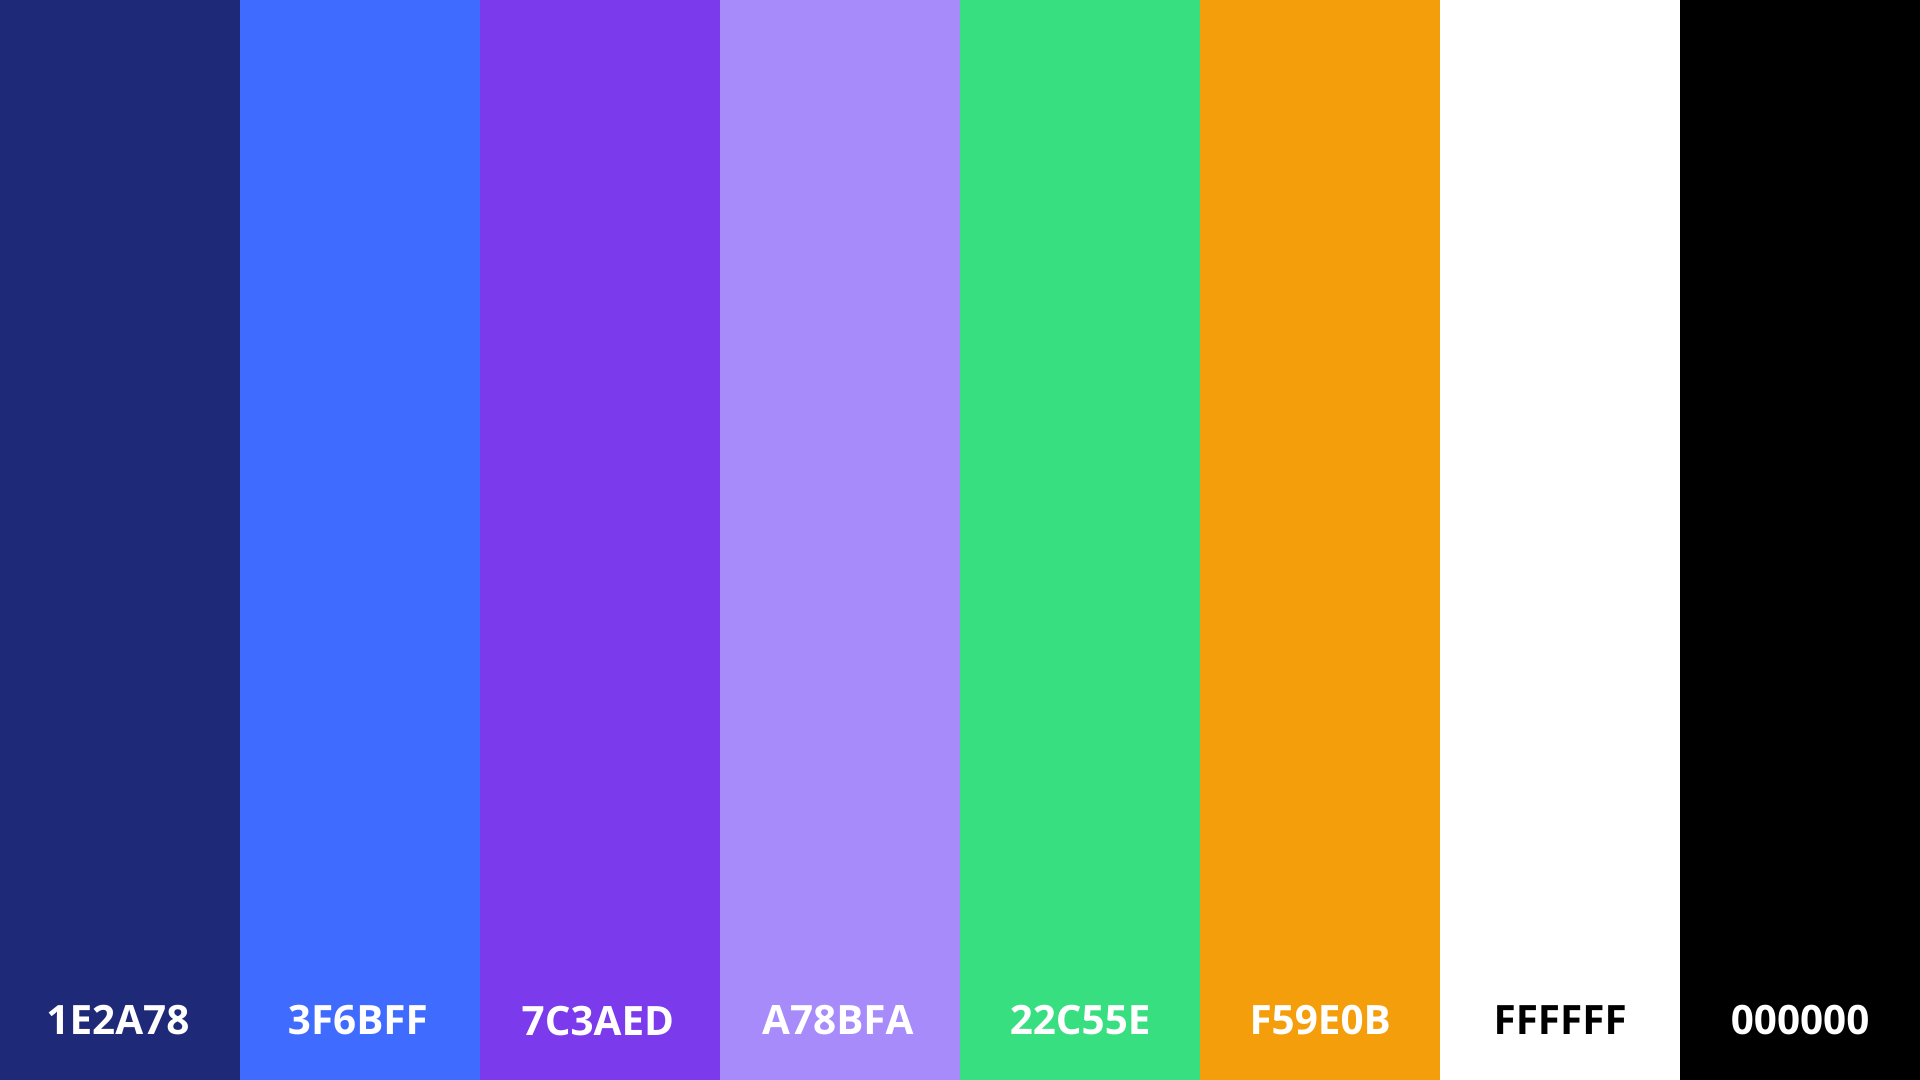
\includegraphics[width=0.92\textwidth]{images/paleta-aiva.png}
  \caption{Paleta de Colores -- Fuente: elaboración propia}
  \label{fig:paleta-aiva}
\end{figure}

\subsection{Logo}
El signo marcario combina un \textbf{símbolo geométrico} (módulos rectangulares que sugieren el trazo de una “A” y la idea de bloques de datos) con el \textbf{logotipo} “AIVA” en tipografía \textit{sans serif} de alta legibilidad.

\begin{itemize}
    \item \textbf{Configuración principal (lockup).} Símbolo a la izquierda y logotipo a la derecha, alineados sobre la línea base. El conjunto se utiliza en positivo (blanco) sobre fondos indigo/azules o en negativo (indigo/violeta) sobre fondos claros.
    \item \textbf{Área de protección.} Mantener un margen libre alrededor del logo equivalente a la altura del símbolo para evitar interferencias con otros elementos.
    \item \textbf{Tamaños mínimos.} Asegurar que el ancho total no sea inferior a 24\,mm en impresos (o 160\,px en pantalla) para conservar la legibilidad de las formas internas.
    \item \textbf{Variantes.} 
    \begin{itemize}
        \item \textit{Monocromo}: uso en una sola tinta (blanco o negro) cuando las restricciones de producción lo requieran.
        \item \textit{Isotipo}: sólo el símbolo para favicons, íconos de app o espacios reducidos.
    \end{itemize}
    \item \textbf{Usos incorrectos.} No distorsionar, rotar ni aplicar efectos de sombra; no alterar la paleta definida; no combinar el logo con fondos de bajo contraste que comprometan la lectura.
\end{itemize}

\vspace{1cm}